\documentclass[article]{IEEEtran}
\usepackage{blindtext, graphicx, biblatex}
\graphicspath{ {images/} }
\addbibresource{references.bib}
\begin{document}
\title{Smart Dust Technology }
\author{by Gerard Naughton }% <-this % stops a space

\maketitle

\begin{abstract}
Text for abstractm.m.
\end{abstract}


\section{Introduction}.\newline
In the fast-paced world of computing, the way we look at and perceive the computer is ever-changing. Once we reach the peak of computing power, data compaction, networking speeds or energy usage, the following day there is a another breakthrough. In the age of the Internet of Things (IoT)\cite{IOT}, the research community are looking for new platforms for obtaining and processing data. The introduction of Smart Dust as a platform may revolutionise this idea. 
The concept of Smart dust is the idea of  “an autonomous sensing, computing, and communication system that can be packed into a cubic-millimeter mote (a small particle or speck) to form the basis of integrated, massively distributed sensor networks”\cite{Mili}. Breakthroughs in engineering and textiles have reduced the size of these motes to cubic millimetres[textiles]. Using this technology with its device size, connectivity and various sensors allows us to interact and monitor the physical world without disrupting it.\cite{MobNet}


\subsection*{History}.\newline
Although smart dust has been mentioned in science fiction dating back to 1973 in a book called “The Invincible” by Stanislaw Lem \cite{lem1973invincible}, it was not until 2001 that the science behind smart dust was first developed in the University of California, Berkley by professors Brett Warneke, Matt Last, Brian Liebowitz and Kristofer S.J Pister. 
Here, they developed how small computing elements and connectivity can reshape the interaction between people and computers. Their project was to explore “whether an autonomous sensing, computing, and communication system can be packed into a cubic-millimeter mote (a small particle or speck) to form the basis of integrated, massively distributed sensor networks“\cite{Mili}. In order for smart dust to be viable they deducted that advances in miniaturization, integration and energy management would be needed. 


\subsection*{What makes up a Mote?}.\newline
Here we see what components are needed to create a mote. 
Figure 1 shows a diagram of a mote. Firstly, the mote will require a power system. That is supplied by a thick film battery, a solar cell and a capacitor. Currently this technology allows us to store 1 joule per cubic millimetre. The solar cell produces 1 joule per day per square millimetre. 
The next requirement will be an integrated circuit which will process sensor data, communication, data storage and energy management. This will be the brain of the mote. 
A photodiode is used to receive communication from other devices. This is achieved through radio wave pulses or infrared light pulses, as used in everyday devices such as remote controls. 
Transmission of data is executed in either of 2 ways; passive transmission using a corner cube retroreflector or active transmission using a laser diode and steerable mirrors.
Having established the main components of the mote it is then time to choose its functionality. Here we choose which sensor technology will be attached to the mote and provide the integrated circuit raw data. Depending on the objective of the mote, various sensors may be used such as light, temperature vibration, magnetic field, acoustic and wind shear.
Finally these wireless motes will not just speak to each other but also to a main base station which can be either 10 metres away or up to a couple of kilometres.  The base station will receive data from the motes and process it into valuable information. Base stations may reside in a computer, hand held device or even in drones\cite{Mili}.

\begin{figure}[h!]
\graphicspath{ {images/} }
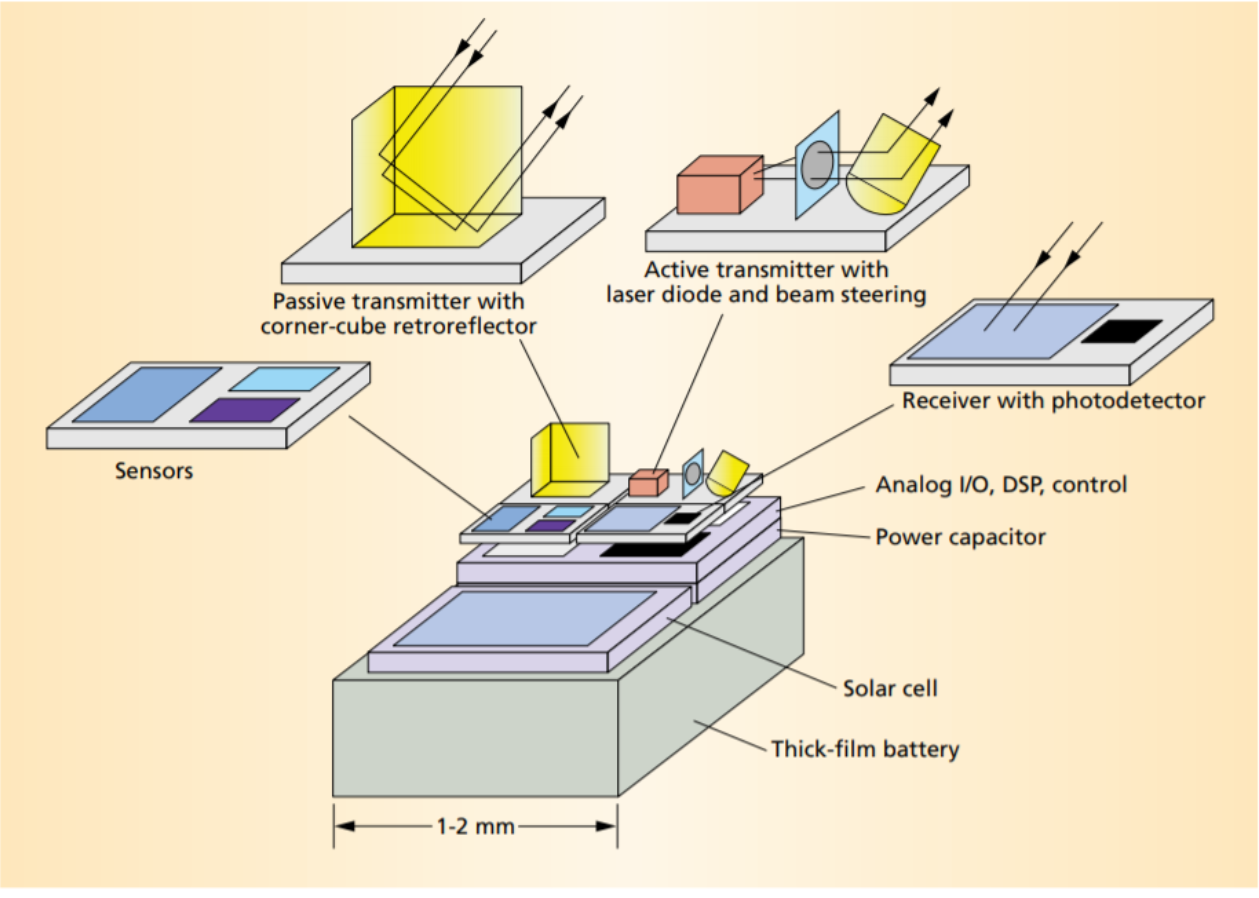
\includegraphics[width=8.8cm, height=6.5cm]{figure1}
\caption{Diagram of a Smart Dust Mote}
\label{Mote Diagram}
\end{figure}


\section{Applications}.\newline

\listoffigures
\printbibliography
\end{document}



